\section{User Modeling}

\textbf{Human vs Computer}

\textit{Strengths of human} \medskip

\begin{itemize}[itemsep=-5pt, topsep=0pt, leftmargin=*]
    \item intuition
    \item memorize cohesive information
    \item signal detection under noise
    \item recognizing complex signals (speech etc.)
    \item recognizing complex configurations (scenes etc.)
    \item adaption to unexpected situations
    \item learniung aptitude
\end{itemize}

\medskip


\textit{Strengths of computer} \medskip

\begin{itemize}[itemsep=-5pt, topsep=0pt, leftmargin=*]
    \item measuring and counting
    \item storing large amounts of incoherent data
    \item detecting known signals
    \item fast and reliable reaction to signals
    \item reliable fatigue free reaction to known signals
    \item superiority if problems can be algorithmically formulated
\end{itemize}

\medskip

\textbf{Model Human Processor} \smallskip


We can look at humans as an information processor. Taking the computers output as input and after processing the information outputting the input for the computer. \smallskip

The humans perception, memory and motor system can be applied to estimate execution time, error rates, training effects for simple stimulation /reaction interactions and system parameters. \smallskip

\begin{center}
	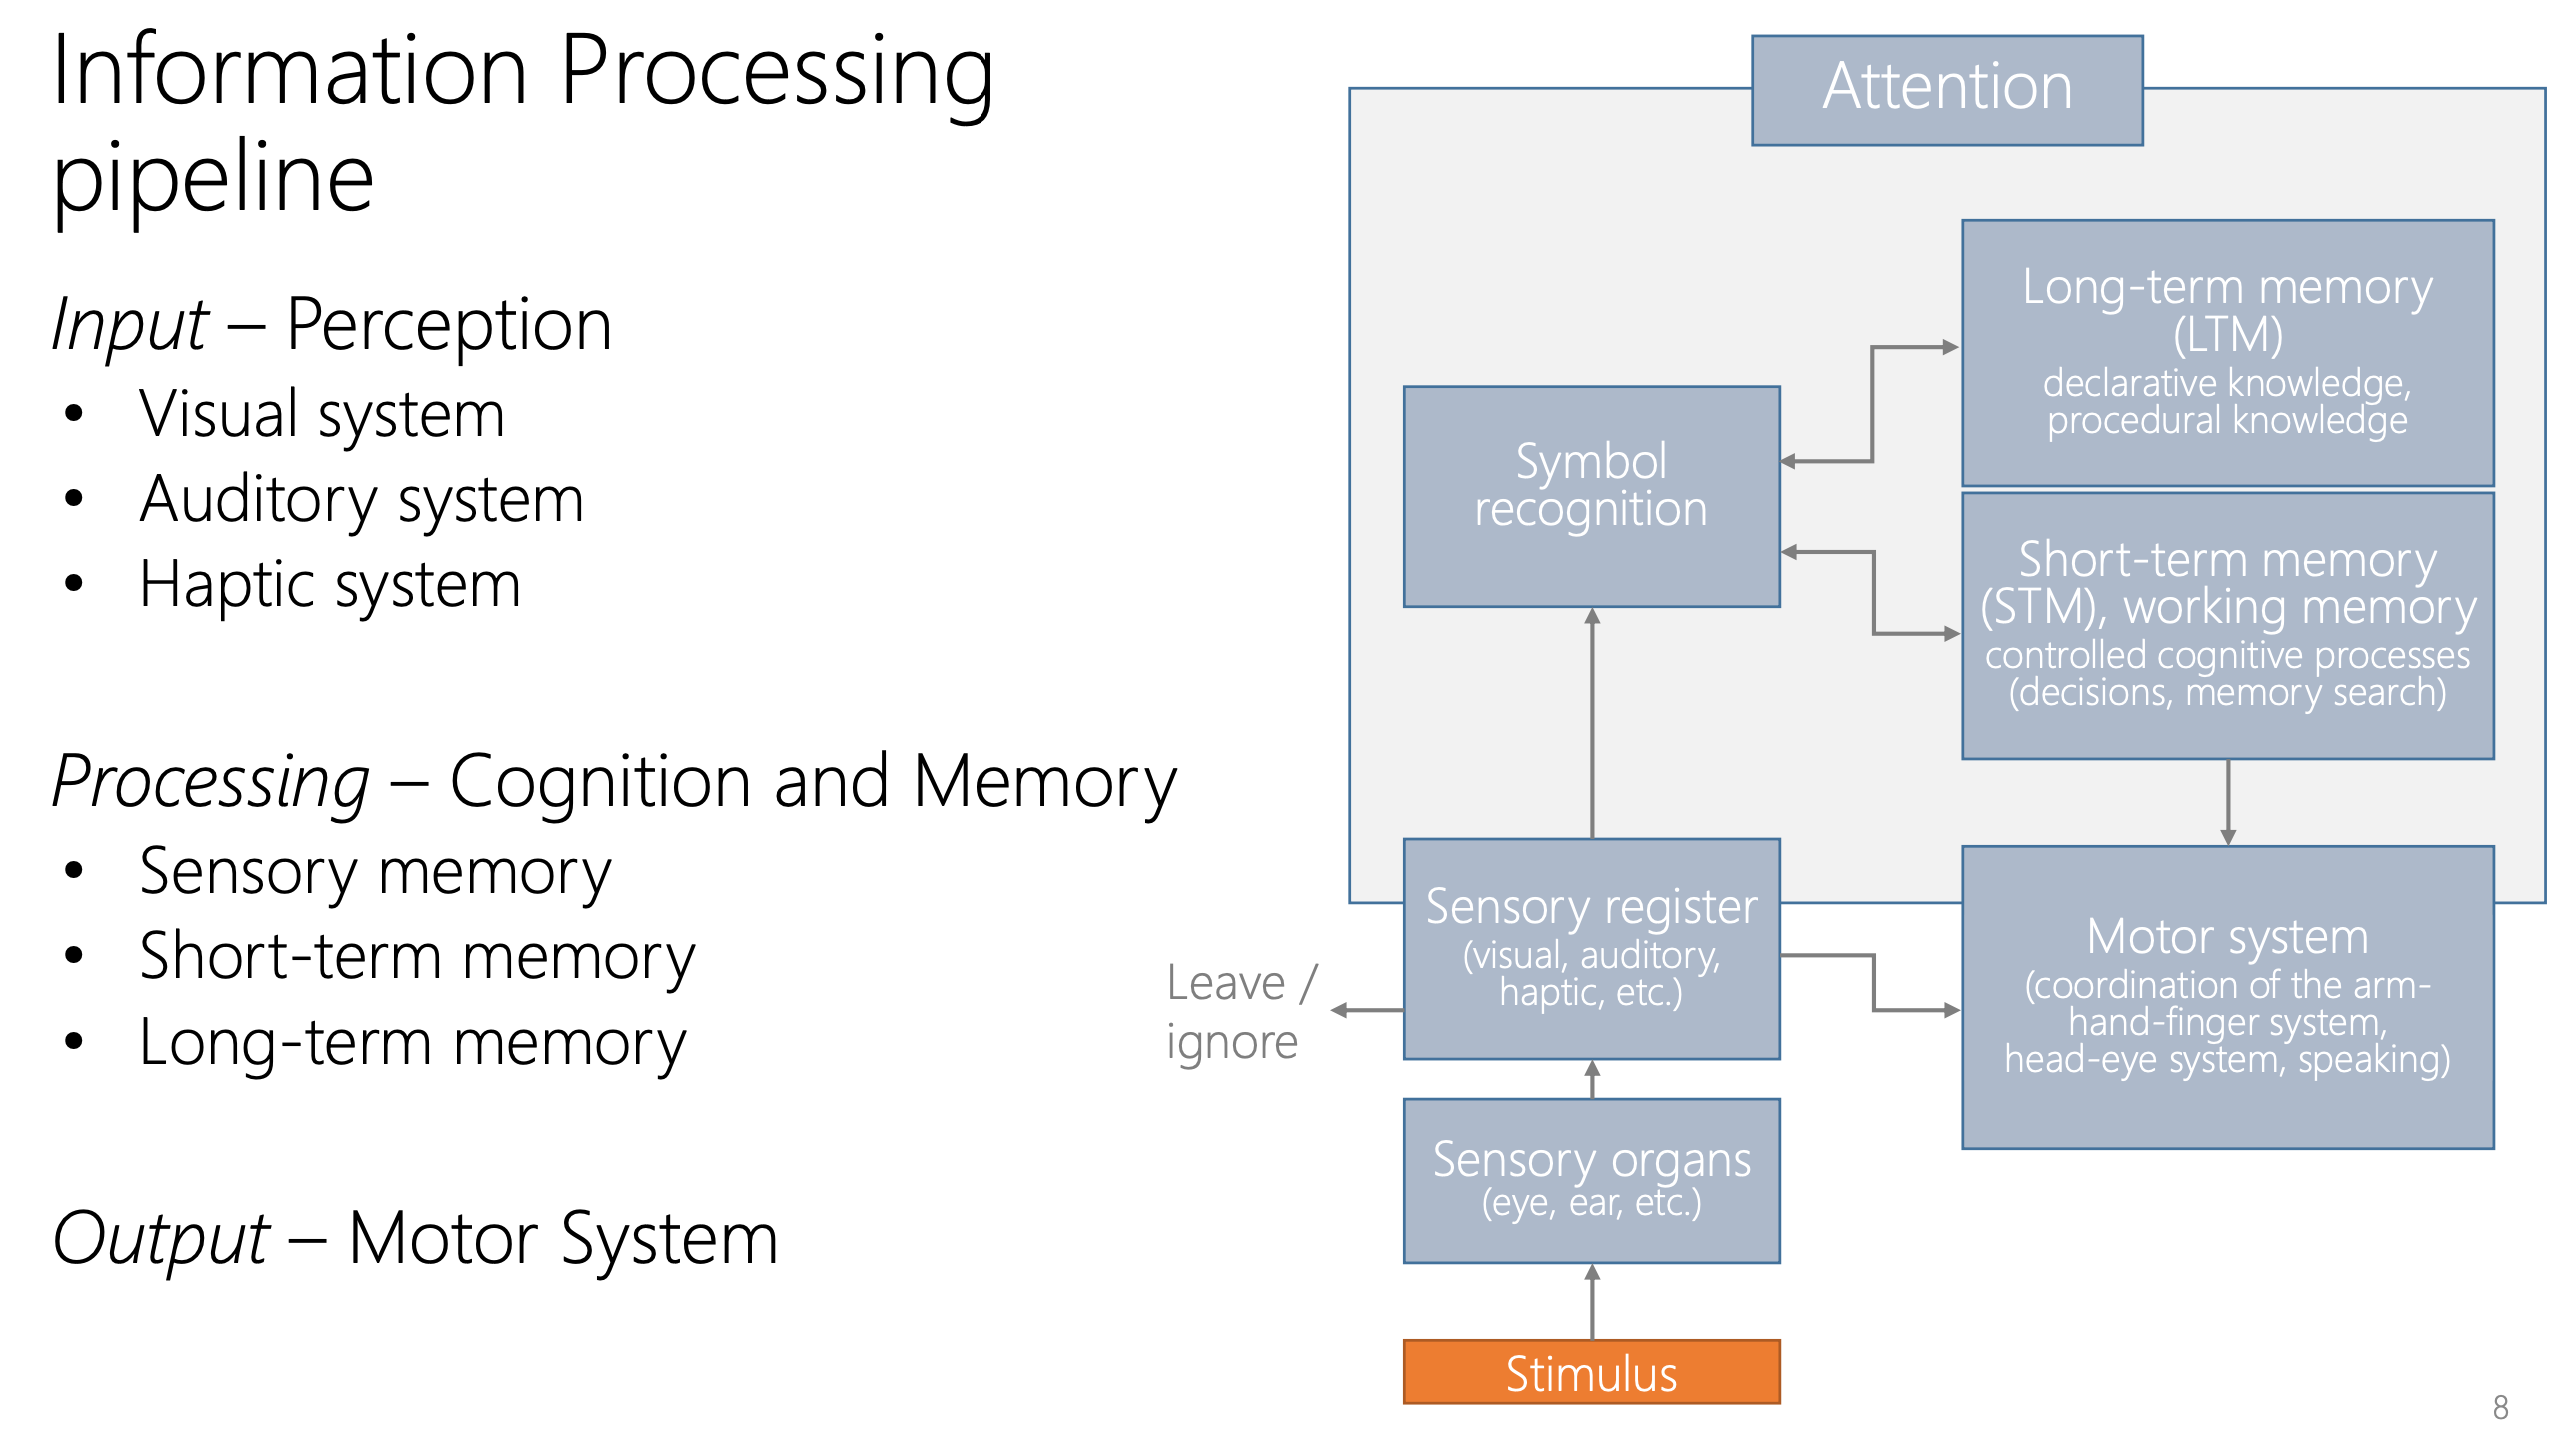
\includegraphics[width=\linewidth]{information_processing.png}
\end{center}

We look at three main processors with associated memory.

\textit{Perceptual System} \smallskip

Containing sensors and buffers. \medskip

\textit{Cognitive System} \smallskip

Containing working memory and content symolically coded \medskip

\textit{Motor System} \smallskip

Contains movements. \medskip

Each processor has associated runtime. Overall runtime is sum of these.  \medskip

\textbf{Perception (Visual System)}


\textit{Anatomy of human eye} \smallskip


\begin{center}
	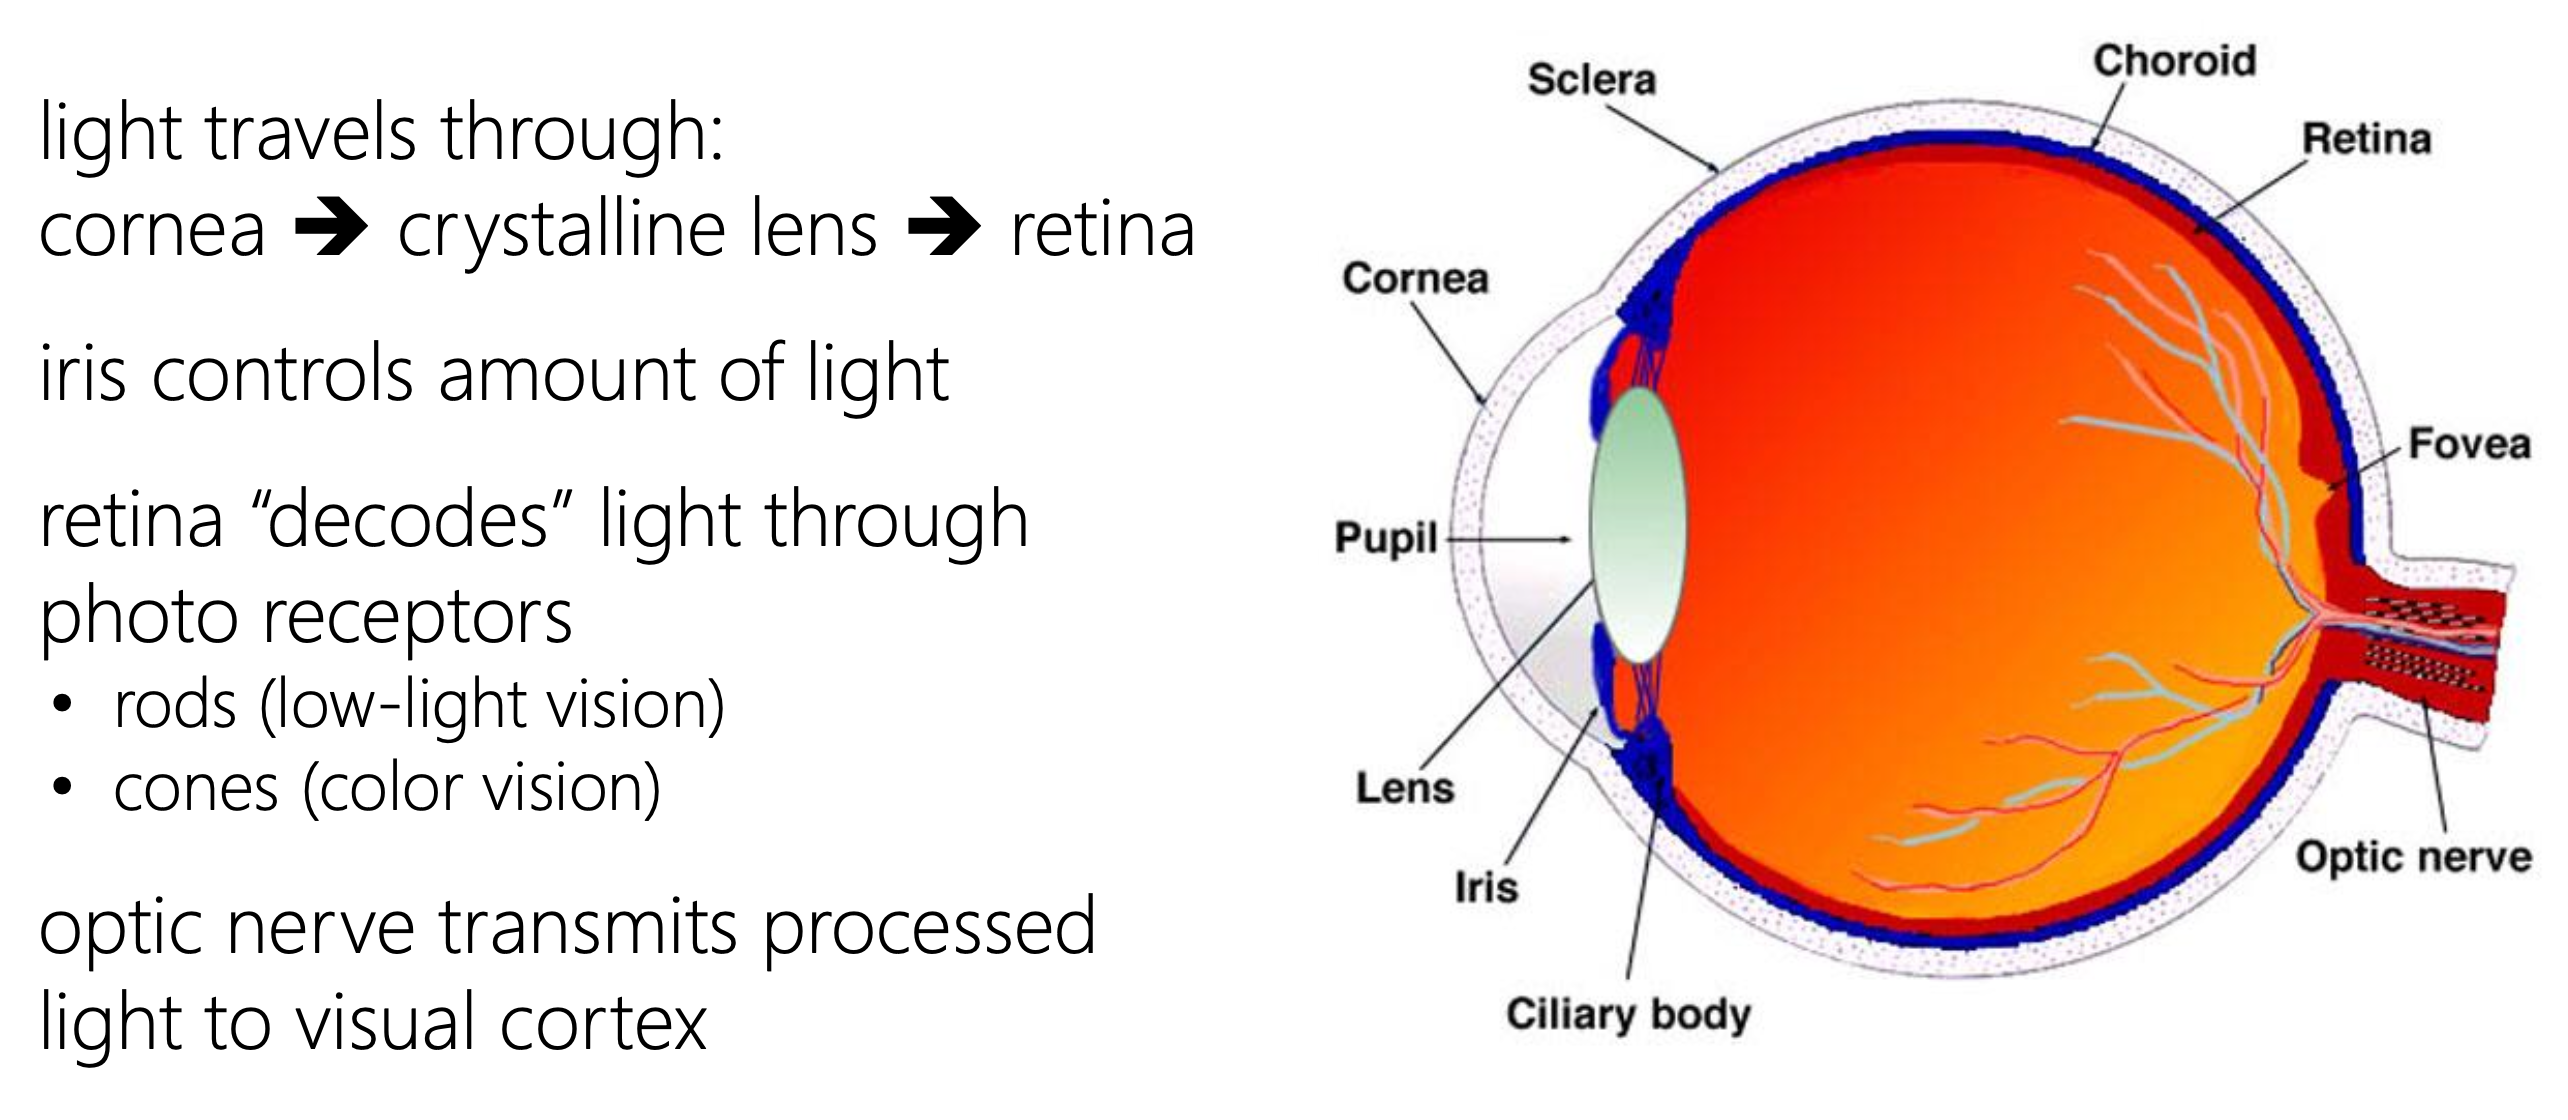
\includegraphics[width=\linewidth]{eye.png}
\end{center}

\medskip

Rods are very light sensitive and have a slow response time. Are located in the periphery of the fovea. 120 million per eye, have maximum sensitivity at 500nm. \medskip

Cones are fast in responding and concentrated at the fovea. 6 million per eye. Three types for blue (S type, 420nm), green (M type, 534nm) and red (L type, 564nm). \medskip


\textit{Visual Field} \smallskip

Sharp vision withing 2 degree radius of fovea. Fine detail. Peripheral vision has decreased visual acuity with distance from fovea. Horizontal visual field is 60 degrees nasally and 90 degrees temporally. Verticual visual field is 60 degrees up and 70 degrees down. \medskip

Useful field of view is rather small (1-4 degrees for high character density and max 15 degrees for low character density.) We use this in Foveated Rendering to reduce details in the outer parts (for instance with eye tracking). \medskip

\textit{Eye movement} \smallskip

Saccades are repositioning of fovea. The take around 30ms with an amplitude of max 600degrees per second. Perception is greatly decreased.\medskip

Fixations are dwelling on one point. Its between saccades. It takes around 90 percent of the visual time. Take around 150 to 600 ms. \medskip

Gaze mvoements are context dependent of foreknowledge, attitute, task and predisposition. \medskip

\textit{Reading} \smallskip

Reading is a sequential loop of fixation and saccades. In average around 230ms fixation and 30ms saccades. On average around 300 WPM reading speed. \medskip

\textbf{(Visual) Attention} \smallskip

We have great gaps in our perception. Interpretation is much sparser than one might assume. Perception of obkects requires lots of attention. Attention has to be directed. \medskip
Perceptual processor receives and buffers signals. One buffer per sensory channel. Perception time is around 100ms (ranging 50-200ms). \medskip

\textit{Bloch's law} \smallskip

$$R = I * t$$

Where R is response, I is intensity and t is exposure time. For t < 100ms, we asusme R constant. As a consequence we have limits on frame-rates (min 10Hz). \medskip

\textbf{Cognitive Processor} \smallskip

Connects perceptual system to motor system. Learning, retrieval of facts, decision making, problem solving etc\dots \medskip

Processing time is around 70ms (25-170). Operates on chunks of information. For instance age, parts of a phone number. \medskip

\textit{Short term memory} \smallskip

Working memory, responsible for intermediate products of thinking and representations of perceptual system. Holds activated item from long term memory. Capacity is limited to 5-9 units (augmented by LTM). Pure capacity is aroun 2-4 units. Decay rate and capacity can be varied depdending on strategy etc. but decreases strongly with increased items. \medskip

\textit{Long term memory} \smallskip

Declarative (facts etc.) and procedural (how to do stuff) parts. Practically unlimited capacity with no decay time. Retrievel depends on associations with for instance eyternal stimuli. It is fast-read, slow-write. 

\textit{Designing for memory} \smallskip

We try to deign for memory through grouping of related functionalities and use familiar structures. We also use recognition instead of recall. \medskip

\textbf{Motor Processor} \smallskip

The average processing time is the sum of time needed for the perceptual, cognitive and motor processor. We differentiate between an open (no perceptual control, motor processor takes around 70ms) and a closed loop (perceptual system controls movement, ca 250ms). \medskip

\textit{Fitt's Law} \smallskip

Models throughput in aimed movements such as reaching for a control in the cockpit or clicking on icons with a mouse. Is very powerful and widely used. Holds in many circumstances, also under water and intoxicated. Allows for comparison among different experiments. \medskip

Originally the task was to touch the centerplate with a pencil, without touching the error plate on the sides. Generally the task is to predict the time to hit a target as a function of distance and size. \medskip

Index of difficulty
$$I_D = log_2(2D/W)$$

\textit{Index of Performance or Throughput} \smallskip

ID = information (nr of bits) required to specify movement (amplitude within given tolerance)\smallskip
IP is index of performance. 

$$IP = ID / MT $$(is in bits/sec)
Depends on input device and limb. \smallskip
Movement time MT

$$MT = a + b * ID$$
$$MT = a + b *log_2(2D/W)$$

In the end we can use the different MTs to estimate a regression on ID and MT (estimate a and b of line). \medskip

\textit{Fitt's Law implications} \smallskip

We find that doubling the distance adds roughly a constant to execution time (Logarithmic nature of the law). Doubling the target width is roughly equal to halving the distance (implicated by D/W term in the formulation). \medskip

\begin{center}
	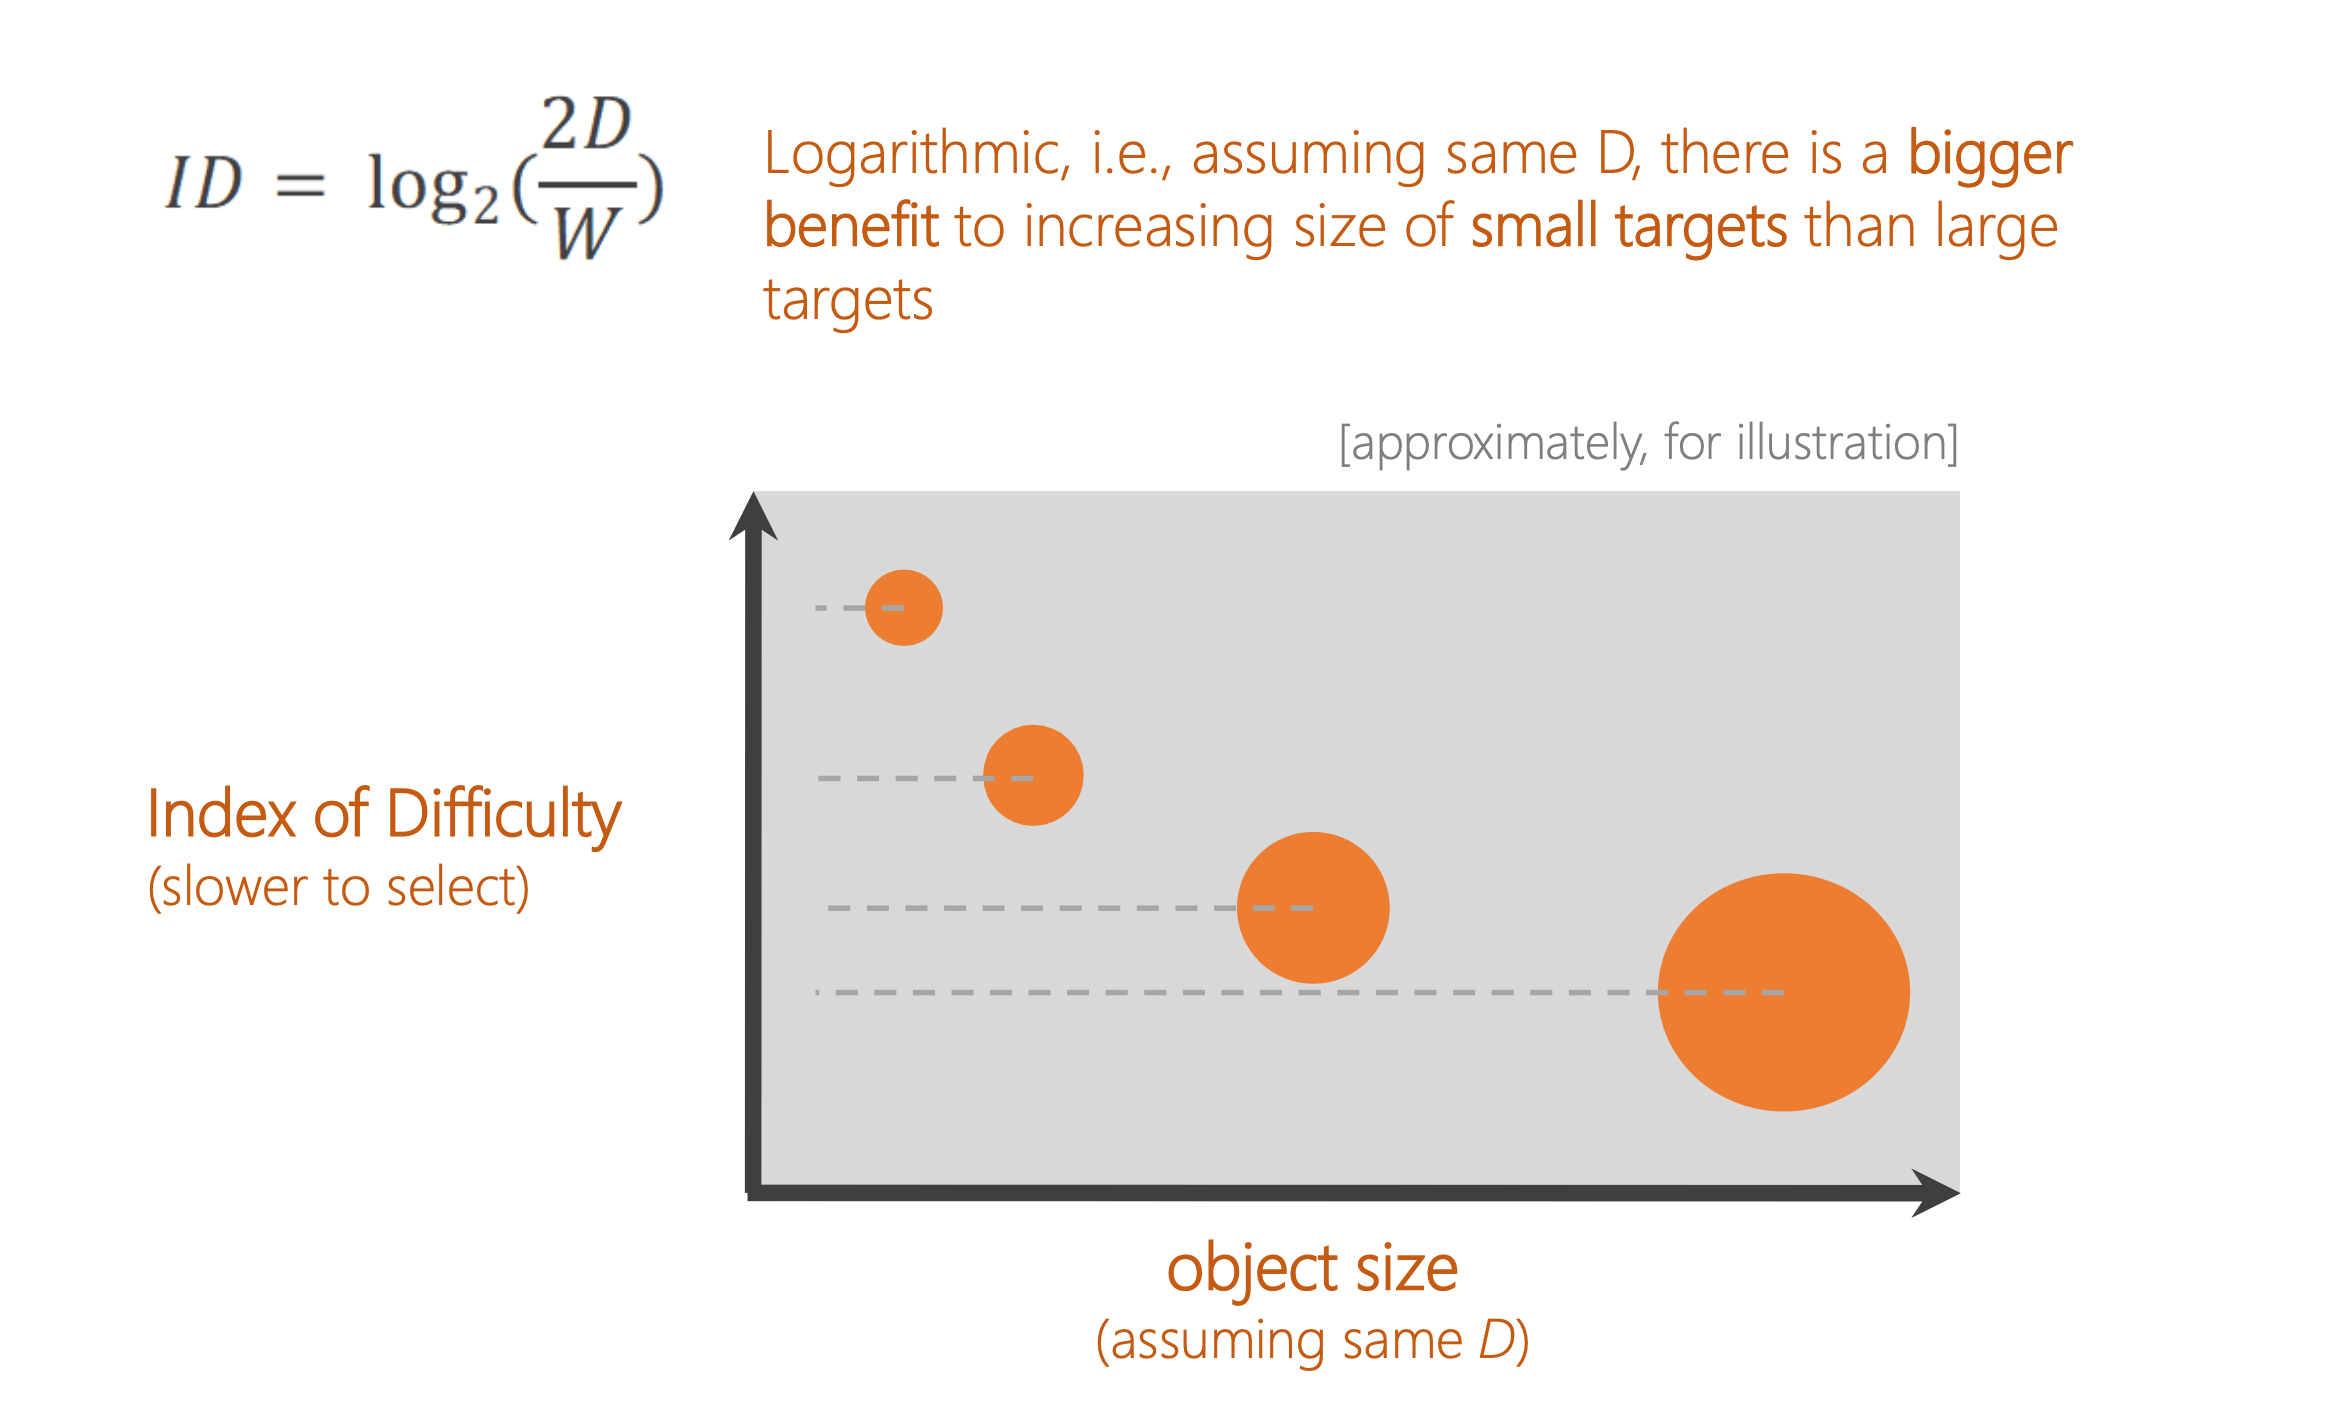
\includegraphics[width=\linewidth]{fitss_law.png}
\end{center}

\textit{Fitt's Law in practice} \smallskip

We can add the last pixel of buttons on the left side, to increase to effective Width of "almost infinite". \smallskip

Larger fields can be clicked more easily. \medskip

\textit{Application: Compare input devices} \smallskip

Compare mouse, trackball and stylus in speed. Use pointing and dragging as actions. This corresponds to finding $a$ and $b$ in the formula for $MT$. The we can compare the index of performance (throughput). We can then use this information to design an "optimal" UI. \medskip

\textit{Limitations of Fitts' Law} \smallskip

Fits law does not: 


\begin{itemize}[itemsep=-5pt, topsep=0pt, leftmargin=*]
    \item consider body asymmetries (right vs. left hand flexion vs. extension)
    \item address parallelization strategies (use multiple finger, hands)
    \item include any cognitive factors (reaction time, visual search time etc.)
\end{itemize}
\medskip

\textbf{Bandwidth} \smallskip


\begin{center}
	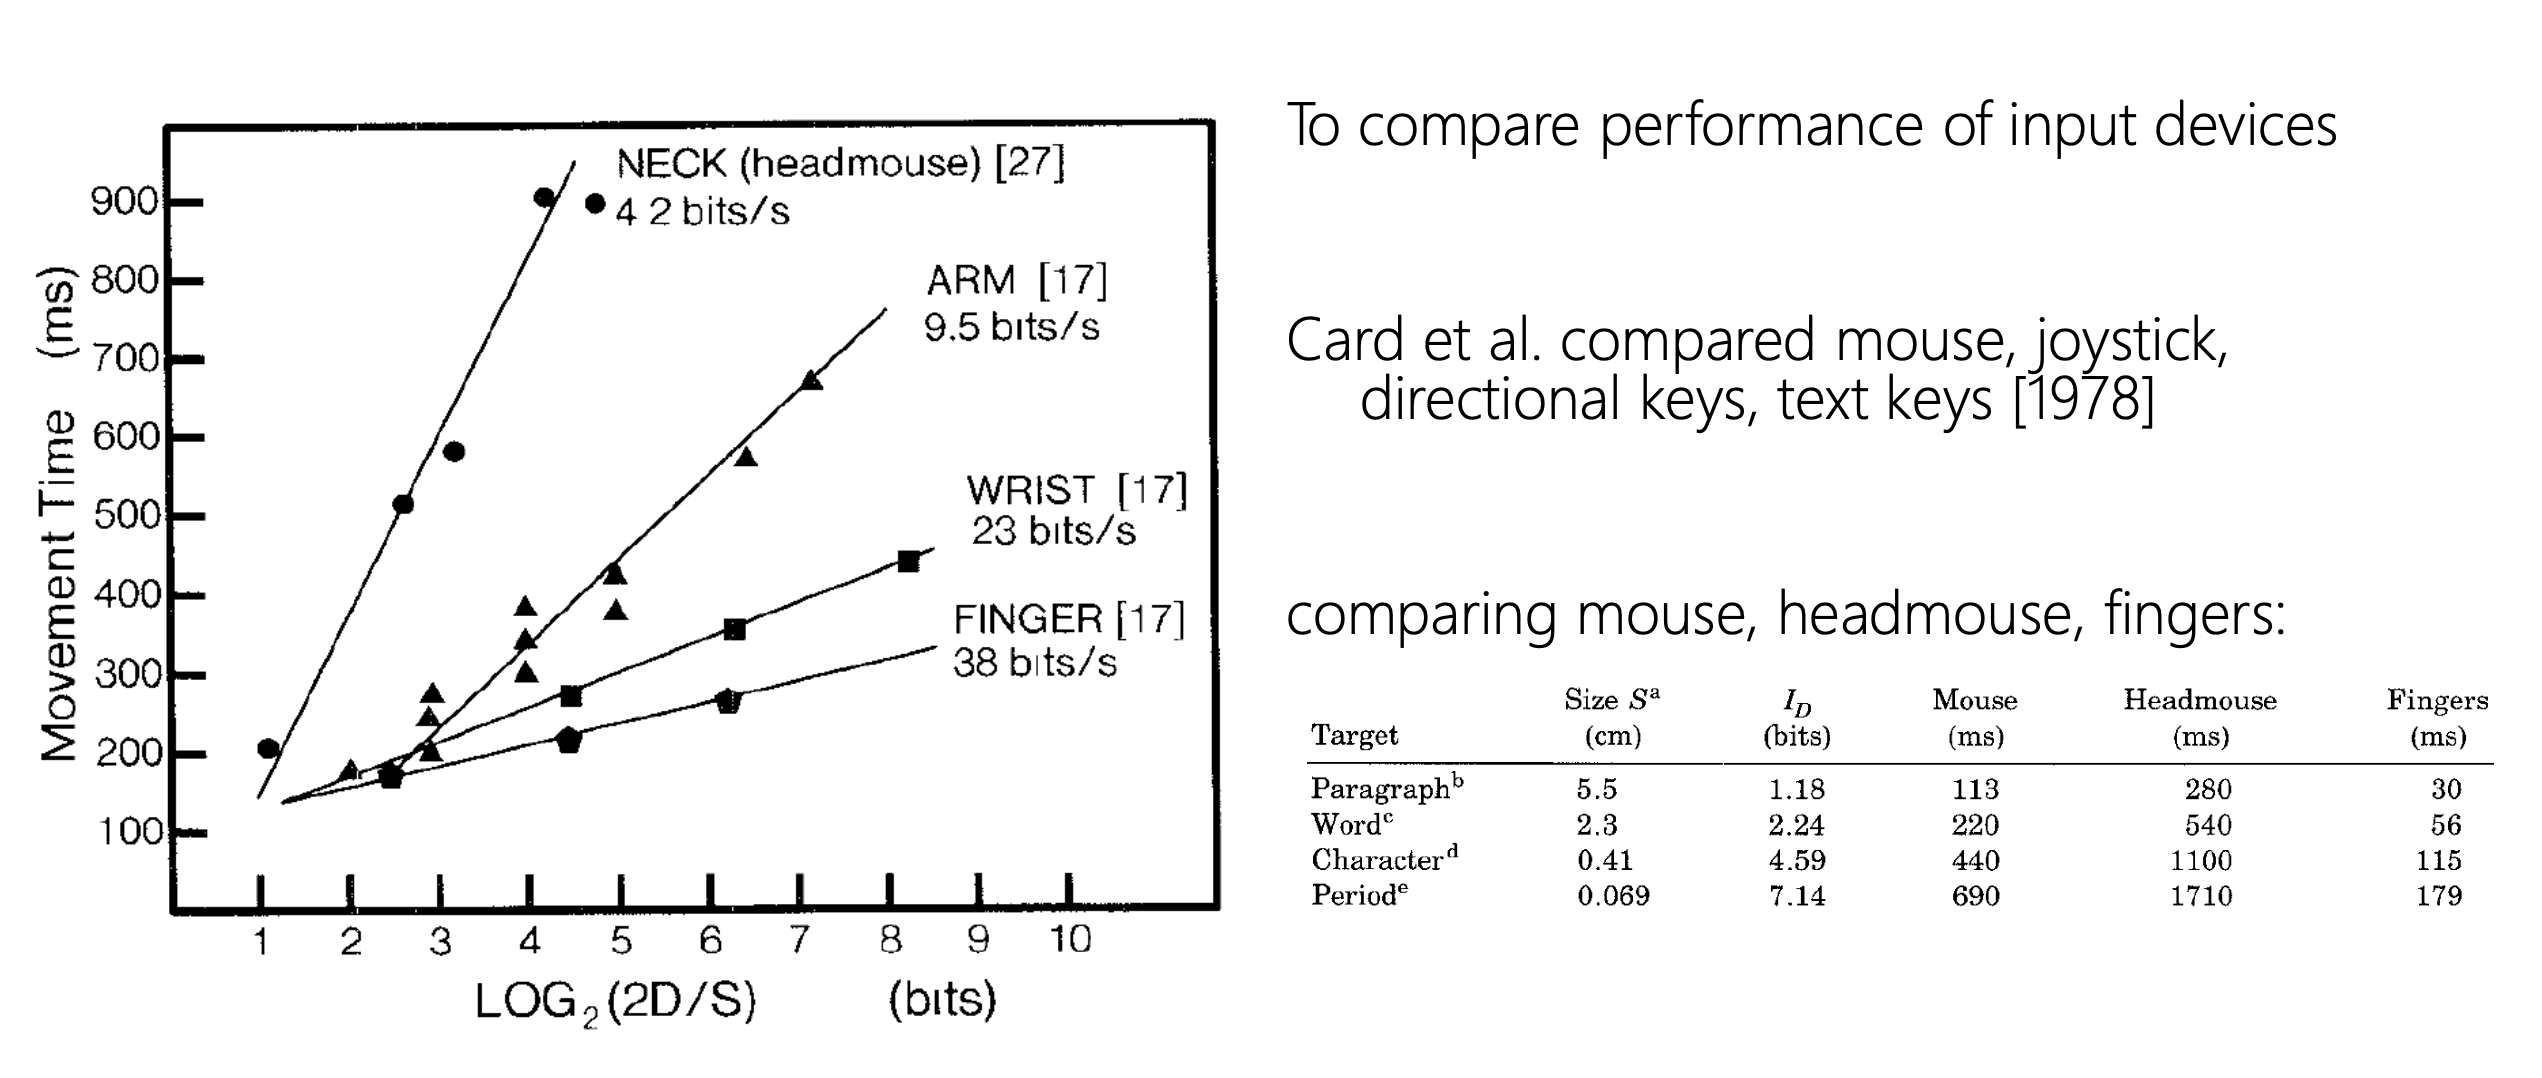
\includegraphics[width=\linewidth]{bandwidth.png}
\end{center}

\medskip

Performance of use depends on human (bandwidth of muscle groups), application (precision requirments of the task) and device (effective bandwidth of input device). \medskip


\textbf{From Model Human Processor to Fitt's Law} \smallskip

\textit{Visual and Proprioceptive Feedback Loop} \smallskip

FIrst we observe handposition, then we plan the movement, we perform the hand movement and finally asses the error to expected position. This is a loop and gets repeated until desired movement is finished. 


\begin{center}
	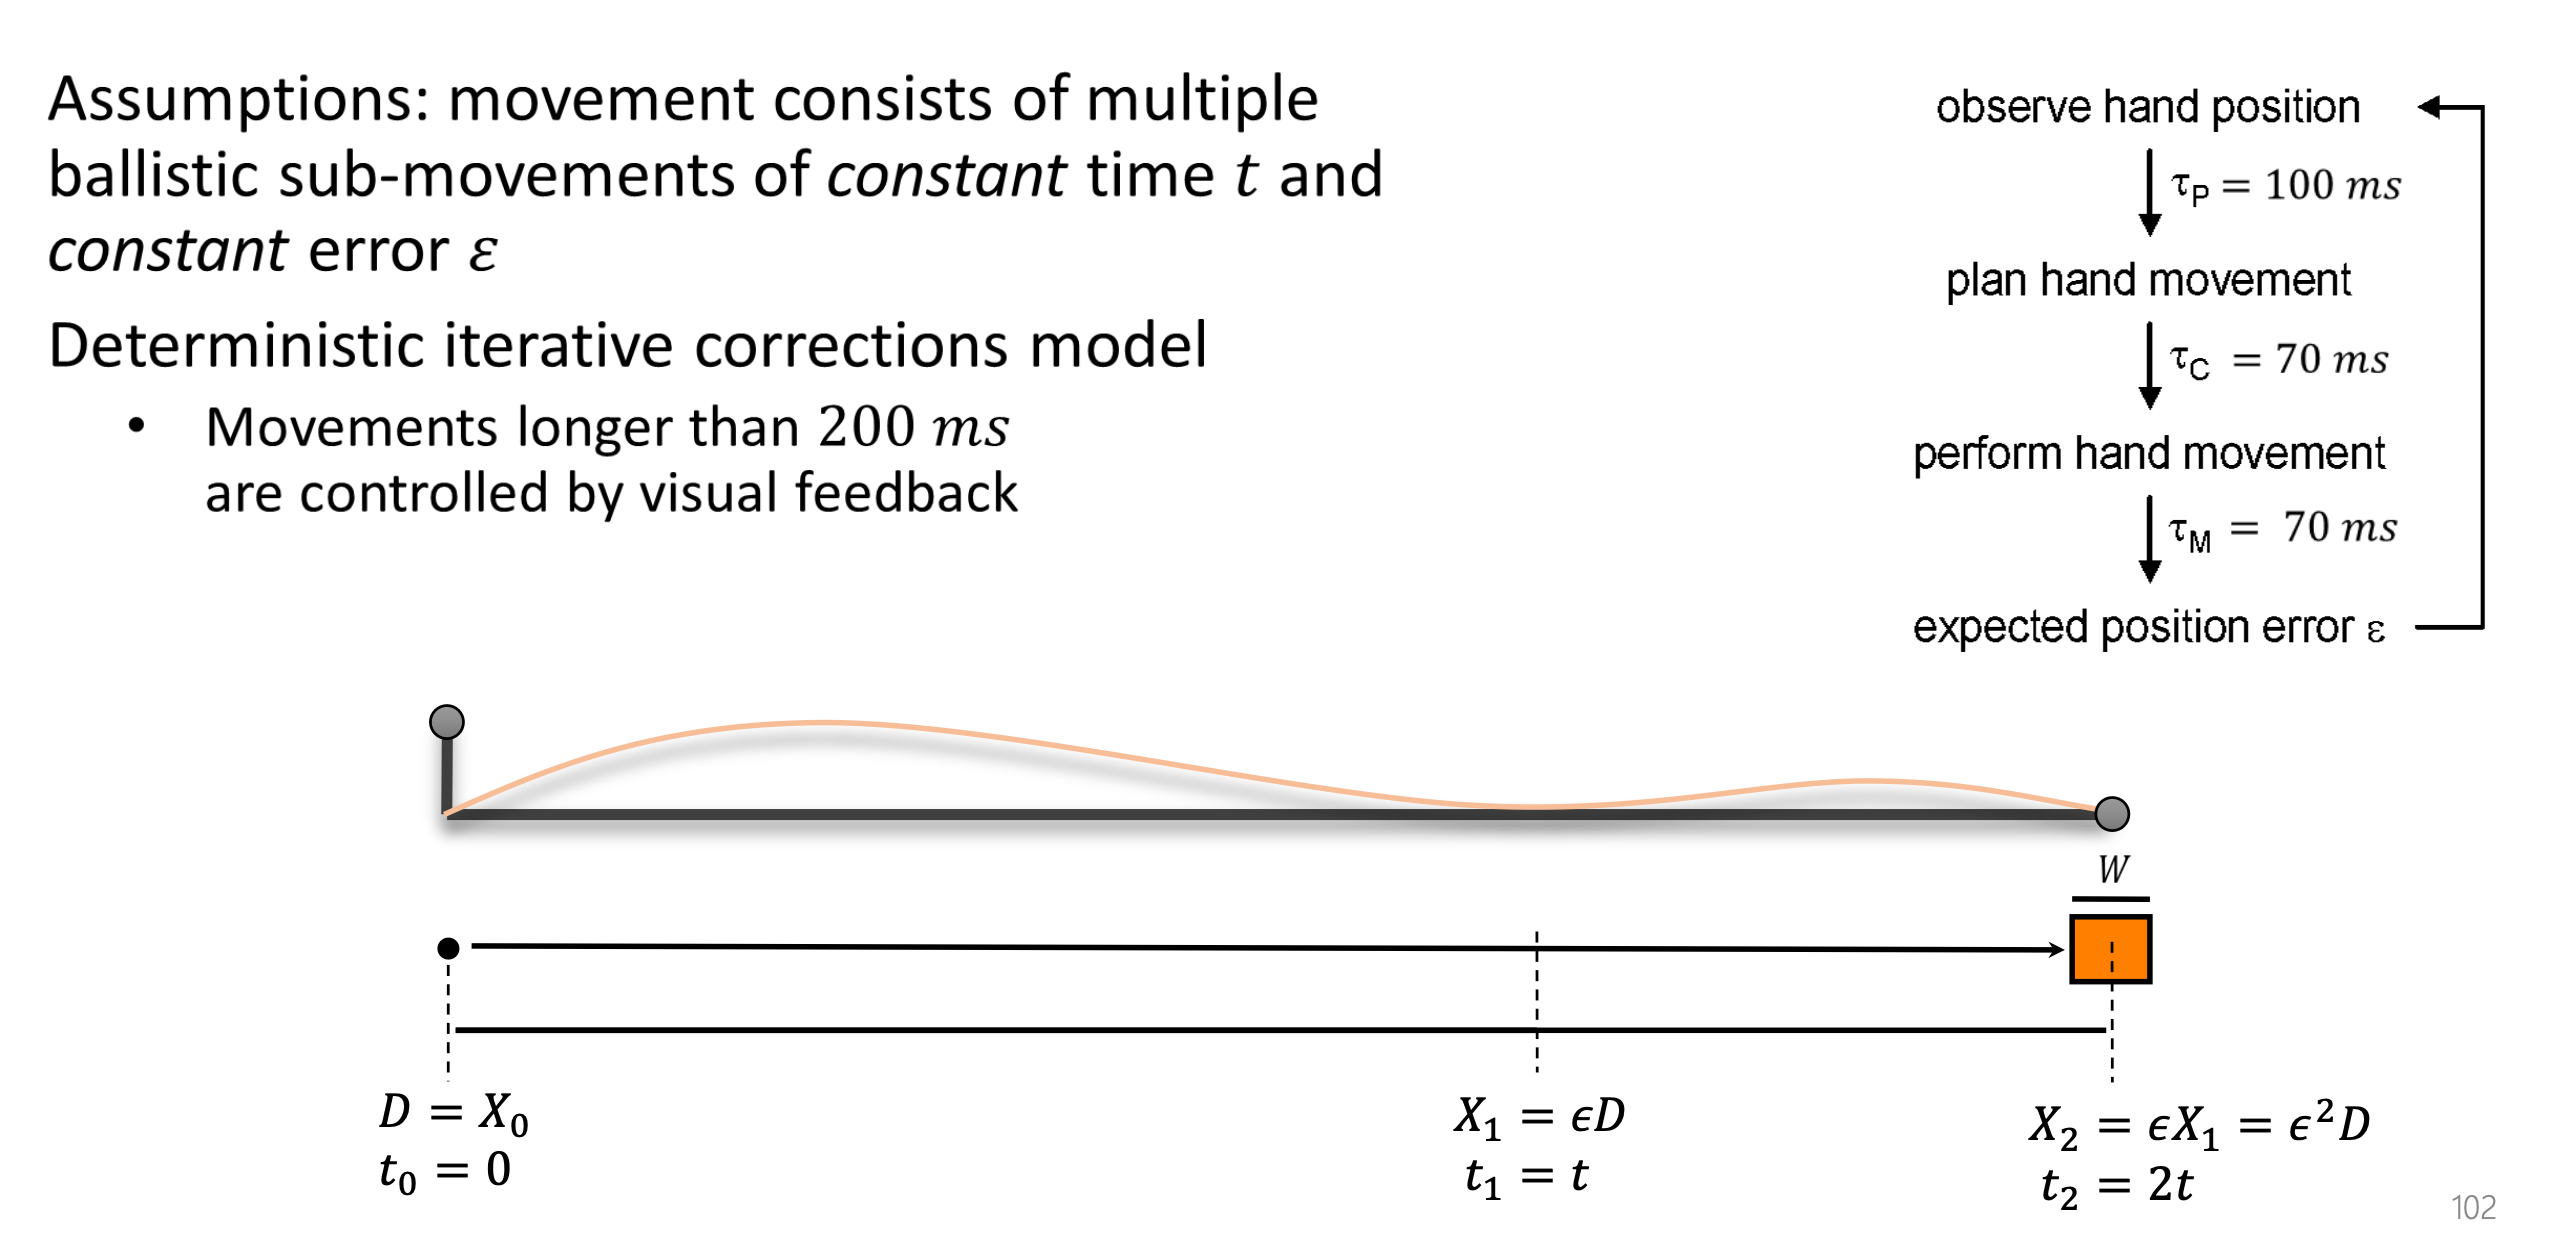
\includegraphics[width=\linewidth]{visual_feedback_loop.png}
\end{center}

We know from MHP that one cycle through all processors is around 300ms. If n is the times we go through loop, the final time then is
$$n \times (\tau_p + \tau_c + \tau_M)$$

After the first cycle we have:
$$X_1 = \epsilon X_0 = \epsilon D$$
In the second cycle:
$$X_2 = \epsilon X_1 = \epsilon(\epsilon X_0)= \epsilon^2 D$$

$n^{th}$ cycle :
$$X_n = \epsilon^n D $$

We stop the movement when:

$$\epsilon^n D \leq \frac{1}{2} W$$

We solve for n:
$$ n = -log_2(\frac{2D}{W})/log_2\epsilon$$

We insert into formula for movement time: 

$$MT = n \times (\tau_p + \tau_c + \tau_M)$$

$\Rightarrow$

$$ MT = \frac{\tau_p + \tau_c + \tau_m}{-\log_{2} \varepsilon} \cdot \log_{2} \left( \frac{2D}{W} \right) $$

$$ MT = I_M I_D $$

$$ I_M = \text{Index of motion} \left( \frac{\text{sec}}{\text{bits}} \right) $$

























